\documentclass{article} % For LaTeX2e
\usepackage{CS2305_submission,times}

% Optional math commands from https://github.com/goodfeli/dlbook_notation.
\input{math_commands.tex}

\usepackage{hyperref}
\usepackage{url}
\usepackage{graphicx}   % for \includegraphics (application figure)
\usepackage{booktabs}   % for the comparison table

% =====================================================================
%  CS2305 Project 3 — Group 17
%  Topic: Von Neumann Architecture vs. Processing-in-Memory (PIM)
%  Structure follows the shared group outline so every member's section
%  slots in consistently.
%  Word budget: main body (Abstract + Sec.1-6, EXCLUDING refs/appendix)
%               must stay <= 500 * 4 = 2000 words.  Per-section budget:
%    Intro ~180 | Definitions ~550 | Relationship ~350 |
%    Applications ~520 | Reflections ~350 | Optional ~130   (~2080 cap, trim)
%  Ownership is marked with % [P1]/[P2]/[P3]/[P4] before each block.
%    P1 = Fan Sitong  : Intro + Von Neumann definition (1.1) + PPT1
%    P2 = Zhang Xiaoyu: PIM definition (1.2) + Relationship (Sec.3)
%    P3 = Chen Yu     : Applications (Sec.4) + Optional case study (Sec.6) + Appendix
%    P4 = You Yining  : Reflections & Conclusions (Sec.5) + PPT2 + talk
%  Placeholder blocks are in \textit{[...]} — replace with real prose.
% =====================================================================

\title{Von Neumann Architecture vs. Processing-in-Memory:\\ Breaking the Memory Wall}

\author{
Fan Sitong \\ Student ID: XXXXXXXX \\ \texttt{x@sjtu.edu.cn}
\And
Zhang Xiaoyu \\ Student ID: XXXXXXXX \\ \texttt{x@sjtu.edu.cn}
\AND
Chen Yu \\ Student ID: XXXXXXXX \\ \texttt{x@sjtu.edu.cn}
\And
You Yining \\ Student ID: XXXXXXXX \\ \texttt{x@sjtu.edu.cn}
}

\newcommand{\fix}{\marginpar{FIX}}
\newcommand{\new}{\marginpar{NEW}}

\begin{document}

\maketitle

% [ALL] Abstract — budget ~110 words. Single paragraph.
\begin{abstract}
For more than half a century the Von Neumann architecture---a processor
separated from memory by a shared bus---has been the foundation of
general-purpose computing. As workloads turn data-intensive, however, the time
and energy spent moving data between memory and processor now dominate, a
limitation known as the \emph{memory wall}. Processing-in-Memory (PIM) responds
by performing computation inside or beside the memory, where the data already
resides. This report compares the two paradigms: it defines each, argues that
PIM is an evolutionary complement rather than a replacement, and surveys where
each fits---Von Neumann for control-intensive general-purpose work, PIM for
data-movement-bound tasks such as AI inference and graph and database analytics.
We conclude that future systems will be hybrid.
\end{abstract}

% =====================================================================
% [P1] Introduction — budget ~180 words
% =====================================================================
\section{Introduction}
For several decades, most general-purpose computers have been designed around the Von Neumann architecture, where a central processing unit executes instructions and exchanges both instructions and data with a separate memory system through shared communication paths. This model has been highly successful because it offers a simple and flexible abstraction for programmers: programs are stored in memory, fetched by the processor, and executed step by step. However, as modern applications become increasingly data-intensive, this separation between computation and storage has become a major performance and energy bottleneck. The core issue is commonly known as the \textit{memory wall}: processor performance has improved much faster than memory latency and bandwidth. As a result, many workloads no longer spend most of their time performing arithmetic operations, but instead waiting for data to move between memory and processors. This problem is especially severe in artificial intelligence, database analytics, graph processing, and large-scale scientific computing, where massive volumes of data must be repeatedly accessed. Processing-in-Memory (PIM), also called near-memory or in-memory computing, addresses this limitation by moving part of the computation closer to, or inside, the memory system. Rather than treating memory as a passive storage component, PIM gives memory a more active role in computation. This survey compares the traditional Von Neumann architecture with PIM, focusing on their basic ideas, their relationship, the problems they solve, and their implications for future computer systems.

\begin{figure}[htbp]
    \centering
    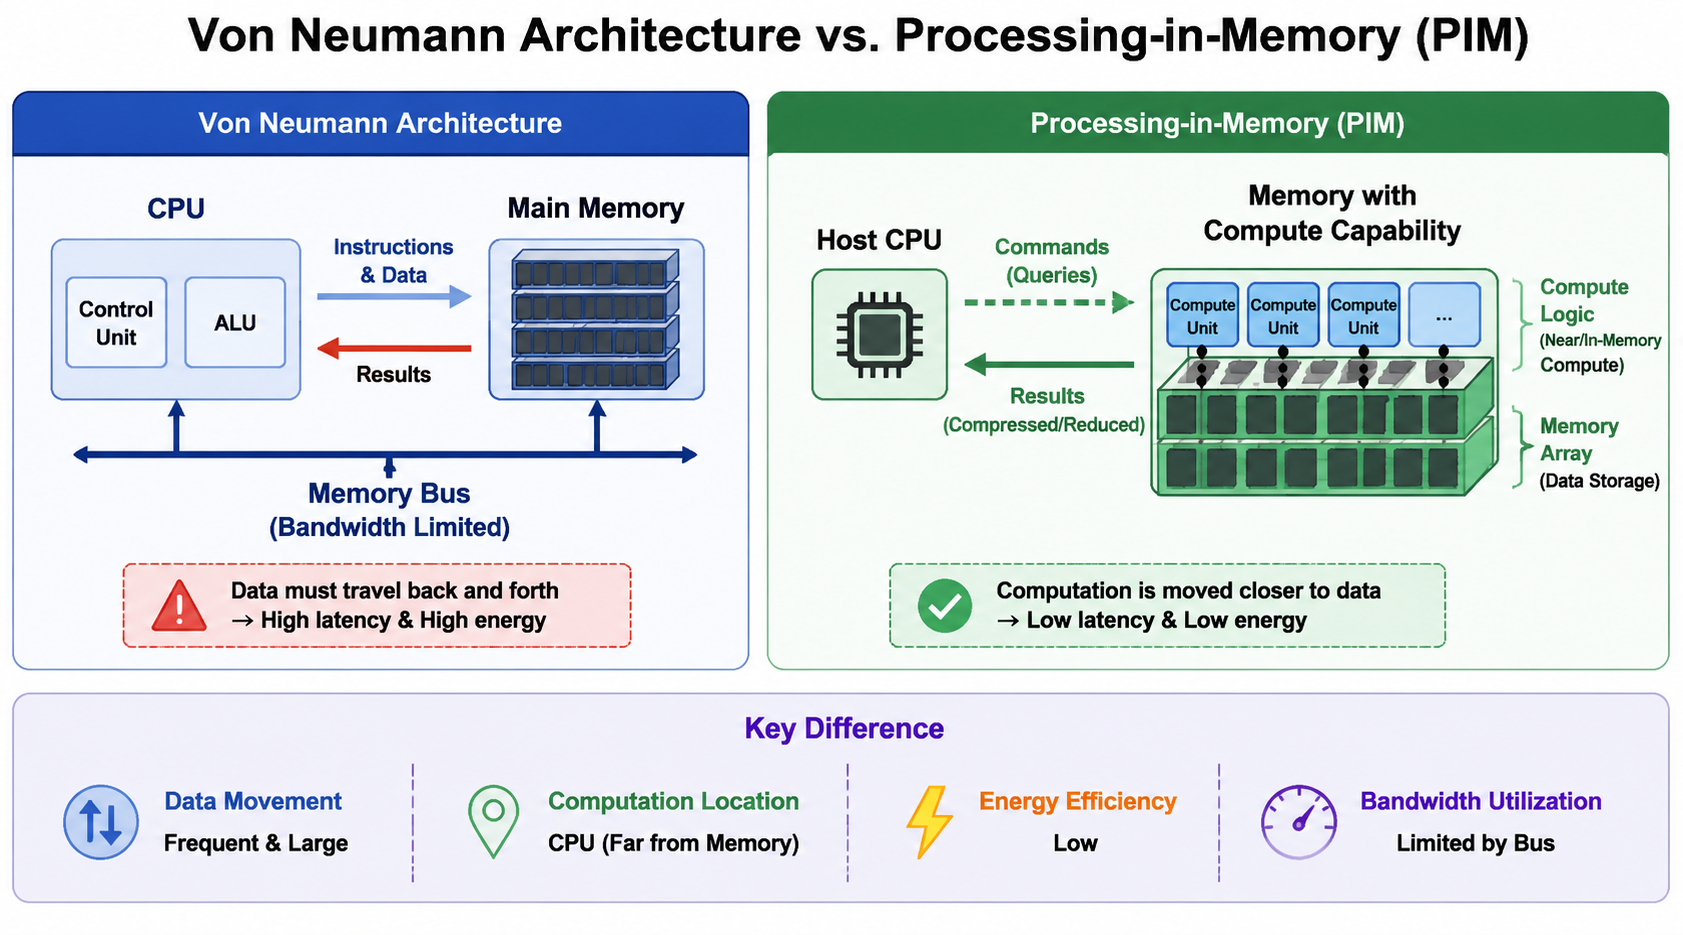
\includegraphics[width=0.9\textwidth]{figure1.png} % 或 figure1.pdf/jpg 根据你文件格式
    \caption{Comparison between the traditional Von Neumann architecture and Processing-in-Memory (PIM). The left panel illustrates the CPU and memory separated by a memory bus, highlighting the bandwidth bottleneck, while the right panel shows PIM moving computation closer to memory, reducing data movement and energy consumption.}
    \label{fig:figure1}
\end{figure}

% =====================================================================
% Section: Basic Definitions
% =====================================================================
\section{Basic Definitions}
\label{sec:def}


\subsection{Von Neumann Architecture}
\label{sec:vn}

The Von Neumann architecture is a classical computer organization model in which
a central processing unit communicates with a memory system that stores both
program instructions and data. This design is based on the
\textit{stored-program concept}, where instructions are represented as data in
memory and fetched by the processor for execution \citep{hennessy2017computer}.
Because of this unified memory model, the same memory space can be used for both
program code and data, making the architecture flexible and suitable for
general-purpose computing.

A typical Von Neumann-style system consists of a processor, memory,
input/output devices, and interconnection buses. The processor usually includes
an Arithmetic Logic Unit (ALU), which performs arithmetic and logical operations,
and a Control Unit, which manages instruction fetching, decoding, and execution.
Memory stores both instructions and operands, while input/output devices allow
the system to communicate with the external environment. These components are
connected through system buses that transfer data, addresses, and control
signals between the processor, memory, and peripherals
\citep{hennessy2017computer}.

Although the Von Neumann architecture has supported decades of successful
computer system design, its separation between computation and storage creates a
major limitation. Since instructions and data must be repeatedly transferred
between the processor and memory, system throughput can be constrained by memory
latency and bandwidth. This limitation is commonly referred to as the
\textit{Von Neumann bottleneck} or, more broadly, the \textit{memory wall}
\citep{wulf1995memory}. This bottleneck is one of the main motivations for
exploring alternative architectures such as Processing-in-Memory.



\subsection{Processing-in-Memory (PIM)}
\label{sec:pim}

To alleviate the performance ceilings of traditional computing, Processing-in-Memory (PIM) has emerged as an alternative architectural paradigm that fundamentally redefines the relationship between computation and storage. Instead of adhering to a strict compute-centric model, PIM integrates computational capabilities directly inside or adjacent to the memory subsystem \citep{sebastian2020memory,mutlu2021primer}. The central philosophy of PIM is to shift from a model of bringing data to computation to one of bringing computation closer to data.

PIM architectures fall into two broad categories based on hardware implementation. Near-Memory Computing (NMC) places dedicated processing elements or logic layers in close physical proximity to memory arrays, such as in a logic die beneath a stack of 3D-stacked memory. In-Memory Computing (IMC) performs calculations directly within the memory arrays themselves by exploiting the analogue physical properties of memory devices, enabling computation within structures such as ReRAM crossbars or modified SRAM arrays \citep{ielmini2018inmemory}. The common thread is a shift from a compute-centric to a data-centric approach.

Practical implementations of the near-memory approach are emerging through technologies like High Bandwidth Memory (HBM), where DRAM dies are stacked vertically and connected to a base logic die through silicon vias, providing a location where simple processing elements can be embedded close to the data \citep{kwon2021hbmpim}. For in-memory logic, emerging non-volatile memory technologies such as ReRAM enable analog computation within the memory crossbar itself, accelerating matrix-vector multiplications fundamental to neural networks \citep{chi2016prime,shafiee2016isaac}.

The primary strengths of PIM are twofold. First, it provides access to massive internal memory bandwidth by enabling parallel interaction with the memory bank's wide internal data paths. Second, it significantly reduces energy consumption by eliminating the costly off-chip data transfers that dominate a conventional system's power budget \citep{horowitz2014energy}.

These advantages come with notable challenges. PIM architectures face significant deployment hurdles, including a complex programming model that breaks the traditional single-address-space abstraction, a lack of standard compilation toolchains, required modifications to memory consistency models, and limited generality across control-flow-heavy tasks. Work must be explicitly partitioned between host processors and PIM units, a trade-off that current hybrid systems actively navigate.

\section{Relationship Between Them}
\label{sec:rel}

\subsection{Evolutionary Perspective}

The relationship between Processing-in-Memory and the classical Von Neumann architecture should be viewed through an evolutionary lens rather than as a revolutionary displacement. PIM does not represent a complete replacement for the Von Neumann model; instead, it serves as a crucial architectural complement and extension developed to overcome the physical limitations of traditional systems under contemporary workload pressures.

For decades, the Von Neumann architecture sustained the computing industry due to its clean abstractions. However, the emergence of the modern memory wall---where the energy and time cost of moving data across a chip interface dwarfs the cost of the arithmetic operation itself \citep{horowitz2014energy}---has rendered pure compute-centric scaling unsustainable. This friction is exacerbated by the rise of pervasive, data-intensive applications such as deep learning, large-scale graph analytics, and real-time database processing. In this context, PIM evolves the infrastructure by embedding processing pockets into memory-bound sectors, establishing a symbiotic architectural framework where computation can be dispatched either to the CPU or to the memory depending on data locality. This represents a shift toward a more physically distributed but logically coherent system, evolving the Von Neumann paradigm rather than discarding it.

\subsection{Key Differences}

The fundamental divergence between the two paradigms lies in their data handling philosophy, contrasting a compute-centric approach with a data-centric approach. Von Neumann systems prioritize centralized processing, routing all data blocks through narrow buses to the CPU, which maximizes general programmability but penalizes massive datasets. In contrast, PIM prioritizes data locality, executing operations directly where the data resides to maximize internal parallelism and suppress off-chip communication. This structural pivot alters the underlying energy characteristics, shifting the primary energy driver from expensive off-chip memory accesses toward localized, low-power near-array operations. These trade-offs are summarized systematically in Table~\ref{tab:compare}.

\begin{table}[t]
\caption{Compute-centric (Von Neumann) vs.\ data-centric (PIM) paradigms.}
\label{tab:compare}
\begin{center}
\begin{tabular}{lll}
\toprule
\textbf{Dimension} & \textbf{Von Neumann} & \textbf{Processing-in-Memory} \\
\midrule
Computation location & In a separate CPU chip & In or adjacent to memory arrays \\
Data movement        & Operands travel over a shared bus & Reduced to near-data or in-array access \\
Energy driver        & Dominated by off-chip memory accesses & Dominated by local, near-array operations \\
Bandwidth            & Pin- and bus-limited & Massive internal parallelism in memory \\
Programmability      & General-purpose, mature ecosystem & Specialized, requires new programming models \\
Best workloads       & Control-intensive, OS, general logic & Data-intensive (AI, graphs, databases) \\
\bottomrule
\end{tabular}
\end{center}
\end{table}

In the Von Neumann model, computation is centralized in a CPU and data must travel across a bandwidth-limited bus. Energy is largely consumed by moving operands between off-chip memory and the processor \citep{horowitz2014energy}. The programming model is a major advantage: decades of toolchain and software stack development make it a flexible, universal target for virtually any algorithm, particularly those dominated by complex control flow.

In contrast, PIM distributes computation to the memory. By operating directly on data where it is stored, it unlocks the memory system's enormous internal bandwidth and avoids costly data transfers. This makes PIM ideal for highly parallel, data-intensive workloads. The cost of this efficiency is programmability and generality. A PIM module's instruction set is often leaner, and effectively using it requires explicit management of data placement and task offloading, breaking the seamless abstraction of a single, flat memory space.

\subsection{Hybrid Architectures}

Driven by these distinct trade-offs, the cutting edge of modern computer engineering lies in the deployment of hybrid and heterogeneous architectures. Rather than abandoning Von Neumann principles, modern systems employ a cooperative CPU + PIM design framework \citep{mutlu2021primer}. In these configurations, a standard Von Neumann processor acts as the primary system host, managing complex control logic, OS scheduling, and general-purpose tasks. When the system encounters heavy, data-bound kernels---such as matrix multiplication loops in neural networks or vector updates in graph traversal---the host CPU offloads these specific operations to the PIM-enabled memory stack or accelerator.

A concrete example is an AI training accelerator that couples an HBM stack, where the logic die at the base implements near-memory processing for weight updates and reduction operations, while a conventional CPU orchestrates the overall training loop. This heterogeneous synergy allows the system to achieve an optimal balance: maintaining the high programmability and mature ecosystem of the Von Neumann model for general applications, while exploiting the high-bandwidth, energy-efficient scaling of PIM to handle the massive datasets of modern computing. The future computing landscape points not toward a single victorious architecture but toward a deep, collaborative integration of both paradigms.

% =====================================================================
% [P3] Applications and Problems Solved — budget ~520 words  *** REAL ***
% =====================================================================
\section{Application Scenarios and Problems Solved}
\label{sec:app}

\subsection{Problems Addressed}
The central problem is the \emph{memory wall}: for decades processor
throughput has grown faster than memory bandwidth, so performance is
increasingly limited by how fast operands reach the processor rather than by
arithmetic itself~\citep{wulf1995memory}. The cost is also energetic. In modern
chips an arithmetic operation costs only a few picojoules, whereas fetching its
operands from off-chip DRAM costs two to three orders of magnitude more, so in
data-intensive systems data movement---not computation---dominates energy and
latency~\citep{horowitz2014energy}. Bus and pin limits compound the effect. PIM
attacks these problems directly by computing where data already lives, removing
much of the traffic the bus and cache hierarchy struggle to
sustain~\citep{sebastian2020memory,mutlu2021primer}.

\subsection{Applications of the Von Neumann Architecture}
The classical model remains the right choice for general-purpose and
control-intensive workloads: operating systems, compilers, software
development, and branch-heavy application or transaction logic. Such
control-flow-dominant tasks reuse little data per access and rely on the
model's flexibility and mature ecosystem, so its bandwidth limitation is rarely
the binding constraint. Its weakness appears only once a workload becomes
data-movement-bound.

\subsection{Applications of PIM}
PIM targets exactly those data-intensive workloads. The flagship case is
AI/deep-learning inference, dominated by matrix--vector multiplication: in a
resistive (ReRAM) crossbar, multiply--accumulate is performed in place by Ohm's
and Kirchhoff's laws, so the weights never move; accelerators such as
ISAAC~\citep{shafiee2016isaac} and PRIME~\citep{chi2016prime} exploit this for
large energy and throughput gains. Near-memory designs instead keep digital
logic but move it beside storage---Samsung's HBM-PIM embeds programmable compute
units in an HBM2 stack and raises effective bandwidth for machine-learning
kernels through bank-level parallelism~\citep{kwon2021hbmpim}. Beyond AI, real
general-purpose PIM hardware now exists: the UPMEM system places thousands of
cores inside DRAM and accelerates memory-bound tasks such as database
scan/filter, graph processing (BFS, PageRank), and
bioinformatics~\citep{gomezluna2022benchmarking}. The common thread is a high
data-to-compute ratio. The trade-off is limited precision and device
variability in analog crossbars, and an immature programming model in
near-memory systems, so achievable gains are workload-dependent and demand
careful data mapping~\citep{ielmini2018inmemory}. Figure~\ref{fig:apps}
summarises where each paradigm is applied.

\begin{figure}[t]
\begin{center}
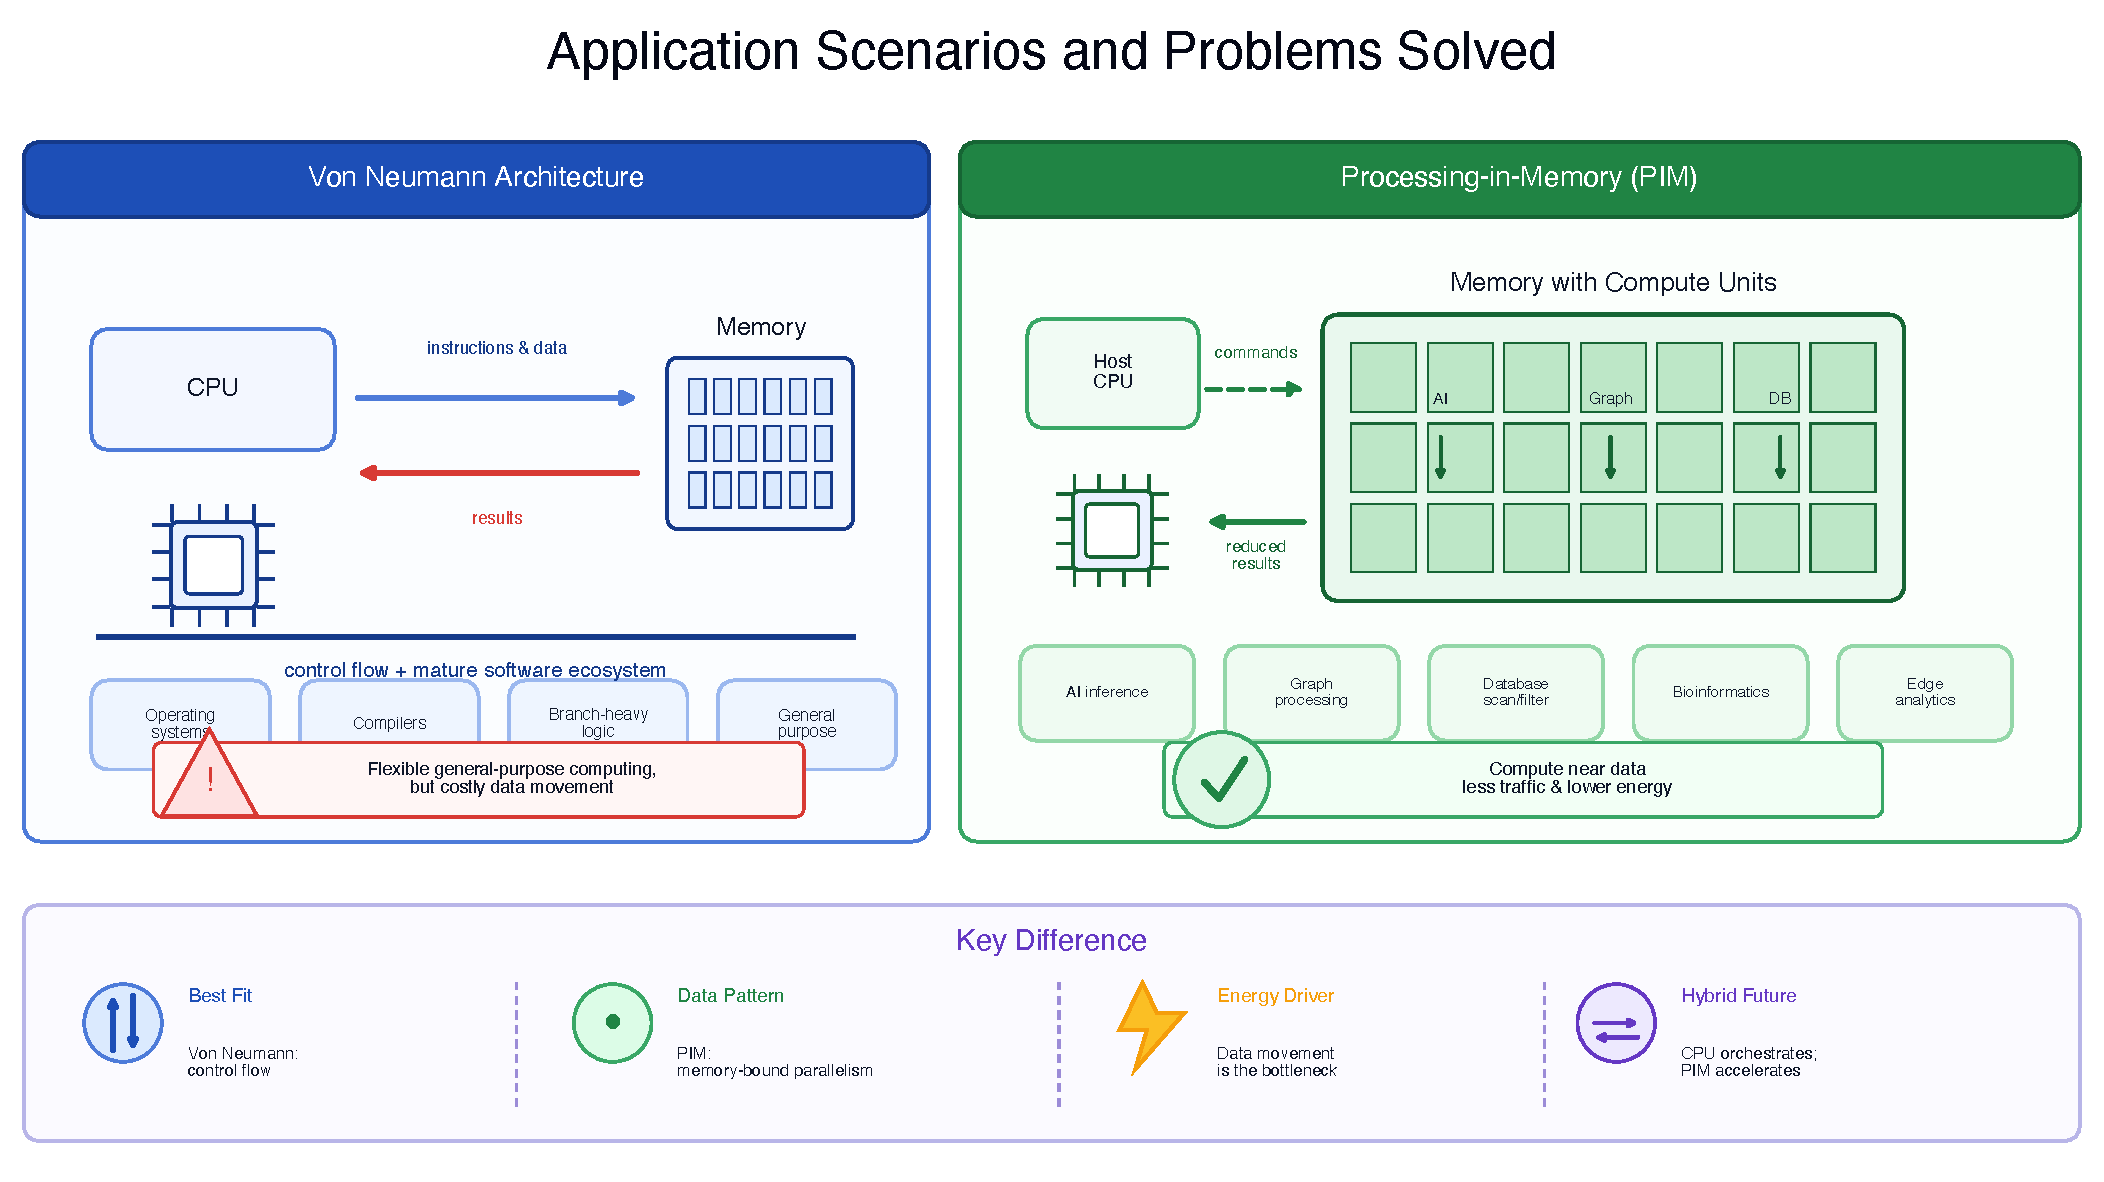
\includegraphics[width=0.92\linewidth]{application_scenarios}
\end{center}
\caption{Application landscape. Von Neumann processors serve control-intensive,
general-purpose workloads; Processing-in-Memory targets data-movement-bound
workloads such as AI inference and edge analytics, where in-/near-memory
execution removes most off-chip data traffic.}
\label{fig:apps}
\end{figure}

% =====================================================================
% [P4] Personal Reflections and Conclusions — budget ~350 words
% =====================================================================
\section{Personal Reflections and Conclusions}
\label{sec:conc}
Our comparison yields a clear insight: the Von Neumann architecture is not
obsolete, and PIM is not a universal replacement. PIM solves one specific,
increasingly dominant problem---the cost of moving data---rather than
computation in general. Where a workload is bound by control flow or reuses
little data, the classical model's flexibility and mature software ecosystem
remain decisive; where a workload is bound by data movement, computing in or
near memory removes the traffic that throttles a conventional system.

The central trade-off is generality versus specialisation. The Von Neumann
model offers a single, flat memory abstraction and a universal programming
target, at the price of the memory wall. PIM offers enormous internal bandwidth
and energy efficiency, at the price of a harder programming model, weaker
generality, and, for analog in-memory designs, limited precision. Because
neither dominates across all metrics, real systems must choose per workload.

Looking forward, we expect heterogeneous, data-centric computing to become the
norm: a Von Neumann host orchestrating general logic while offloading data-bound
kernels to PIM accelerators, as already seen in commercial HBM-PIM products. The
harder bottleneck may be software rather than hardware---without standard
compilers, libraries, and consistency models, PIM's raw hardware gains are
difficult to realise in practice, and AI's appetite for memory bandwidth will
keep driving this evolution.

We therefore conclude that the future is not a single victorious architecture
but a collaborative integration of both: Von Neumann cores and PIM accelerators
coexisting to balance flexibility and efficiency. For us, the most valuable
lesson was learning to reason about computing in terms of data movement and
energy, not merely operation count---a perspective we expect to carry into
future study and work on AI hardware and systems.

% =====================================================================
% [P3] Optional: brief case study — budget ~130 words  *** REAL ***
% =====================================================================
\section{Optional: A Brief Case Study}
\label{sec:case}
A single example makes the contrast concrete. Consider a matrix--vector product
$y = Wx$ with an $N\times N$ weight matrix. On a Von Neumann processor every one
of the $N^2$ weights must be read from memory and carried across the bus to the
ALU to perform one multiply--accumulate, so data movement scales as $N^2$ and
dominates both time and energy. In a ReRAM crossbar the same operation is
computed in place: the weights are stored as cell conductances and the result is
obtained in essentially one analog step via Ohm's and Kirchhoff's laws, so the
$N^2$ weights never move~\citep{shafiee2016isaac,sebastian2020memory}. This one
kernel captures why PIM wins on data-movement-bound work, while the Von Neumann
path wins where data is reused little or control flow dominates.

% =====================================================================
\bibliography{CS2305_submission}
\bibliographystyle{CS2305_submission}

% =====================================================================
% [P3] Appendix — does NOT count toward the word budget
% =====================================================================
\appendix
\section{Appendix}

\subsection*{How was the division of labor structured among team members, and how did the team collaborate (i.e., what were the connections between the divided tasks)?}
Answer: The work was split along the report's logical flow so that each part
fed the next. Fan Sitong wrote the introduction and the Von Neumann definition
(Section~\ref{sec:vn}) and built the first PPT segment; Zhang Xiaoyu defined
Processing-in-Memory (Section~\ref{sec:pim}) and analysed the relationship
between the two paradigms (Section~\ref{sec:rel}), building directly on the
bottleneck described above; Chen Yu surveyed the application scenarios and the
problems each paradigm solves (Section~\ref{sec:app}), added the case study
(Section~\ref{sec:case}) and the figure, and compiled this appendix;
You Yining wrote the reflections and conclusions (Section~\ref{sec:conc}),
prepared the second PPT segment, and delivered the talk. The definitions
(Fan, Zhang) supplied the vocabulary the applications section (Chen) builds on,
and the conclusion (You) draws the whole argument together; members
cross-reviewed adjacent sections to keep terminology and the word budget
consistent.

\subsection*{Why was this topic chosen? (Share the motivations behind the topic selection, such as interest sparked by in-class knowledge or specific reasons for choosing it over other candidate topics.)}
Answer: \textit{[Draft from P3's view; each member to add a sentence:] The
course's treatment of the memory hierarchy and the data-transfer bottleneck
made the ``memory wall'' feel like a live, unsolved problem rather than a
textbook fact. Compared with other candidate topics (e.g.\ RISC vs.\ CISC),
Von Neumann vs.\ PIM pairs a foundational concept every member already
understood with a genuine research frontier, giving both accessibility and
technical depth.}

\subsection*{What is the connection between the selected topic/investigation and the course?}
Answer: The topic sits at the centre of the course. The Von Neumann model, the
CPU--memory bus, and the fetch--decode--execute cycle are core lecture content,
and the memory hierarchy (caches, bandwidth, latency) is exactly what the
``memory wall'' concerns. PIM extends these ideas to a current research
direction, letting us apply course concepts (bandwidth, locality, parallelism)
to evaluate a modern architectural shift.

\subsection*{What is the significance of this investigation for your future research/career?}
Answer: \textit{[Draft for P3; each member should add their own one-line
perspective:] Studying how energy and bandwidth limits reshape architecture is
directly relevant to anyone working on AI hardware, systems, or
energy-efficient computing. The investigation built skills in reading
architecture literature critically and reasoning about hardware--software
trade-offs that transfer to future research and engineering work.}



\end{document}


